\documentclass[11pt, conference]{IEEEtran}
\IEEEoverridecommandlockouts
% The preceding line is only needed to identify funding in the first footnote. If that is unneeded, please comment it out.
\usepackage{algorithm}
\usepackage{algpseudocode}

\usepackage{cite}
\usepackage{amsmath,amssymb,amsfonts}
% \usepackage{algorithmic}
\usepackage{subfigure}
\usepackage{placeins}
\usepackage{graphicx}
\usepackage{textcomp}
\usepackage{xcolor}
\usepackage{lipsum}
\usepackage{hyperref}
\usepackage{float}
\usepackage{booktabs}
\usepackage{multirow}
% \usepackage{subcaption}
\usepackage[OT1]{fontenc} 
% \usepackage{fontawesome5}
\algrenewcommand\algorithmicrequire{\textbf{Input:}}
\algrenewcommand\algorithmicensure{\textbf{Output:}}


\hypersetup{
    colorlinks,
    linkcolor={black},
    citecolor={black},
    urlcolor={blue!80!blue}
}
\def\BibTeX{{\rm B\kern-.05em{\sc i\kern-.025em b}\kern-.08em
    T\kern-.1667em\lower.7ex\hbox{E}\kern-.125emX}}
\begin{document}

\title{Kinodynamic RRT Practice
\thanks{This is the final project for course ROB 422: Introduction to Algorithmic Robotics. The open-source code of the project can be found in  \href{https://github.com/silvery107/motion-planning-practice}{https://github.com/silvery107/motion-planning-practice}.}%
}

\author{
\IEEEauthorblockN{Yulun Zhuang}
\IEEEauthorblockA{\textit{Robotics} \\
\textit{University of Michigan}\\
Ann Arbor, United States \\
yulunz@umich.edu}
}

\maketitle

\begin{abstract}
In this paper, an efficient implementation of the Kinodynamic RRT algorithm and its bidirectional variant are presented. The planners is demonstrated using a planar hovercraft robot to find a path within the maze with a non-trivial set of obstacle walls. The performance statistics is compared in terms of the number of motion primitives, path qualities and the computation time.
\end{abstract}

\begin{IEEEkeywords}
Motion Planning, Kinodynamic RRT
\end{IEEEkeywords}


\section{Introduction}
% Motivate why the problem you are solving is important. What applications require this kind of method?

Motion planning is a fundamental problem in robotics, involving the generation of a feasible path for a robot from a start state to a goal state while avoiding obstacles\cite{lavalle2006planning}. This task becomes significantly more complex in kinodynamic planning, where the robot's dynamics and kinematics are taken into account. Kinodynamic Rapidly Exploring Random Trees (RRT)\cite{lavalle2001randomized}, a variant of the classic RRT algorithm\cite{lavalle1998rapidly}, is specifically designed to handle such complexities. It is particularly relevant in applications where the dynamics of the robot cannot be decoupled from its spatial navigation, such as in autonomous vehicles, and aerial robotics.

In kinodynamic planning, the solution must respect the robot's dynamic constraints and kinematic feasibility\cite{donald1993kinodynamic}. This makes the problem more challenging than standard path planning, as it requires considering the differential constraints in robot dynamics. The key challenge lies in ensuring that the generated path is dynamically feasible, meaning the robot can physically follow the path given its motion capabilities and limitations.


\begin{figure}[htb]
    \centering
        \textsf{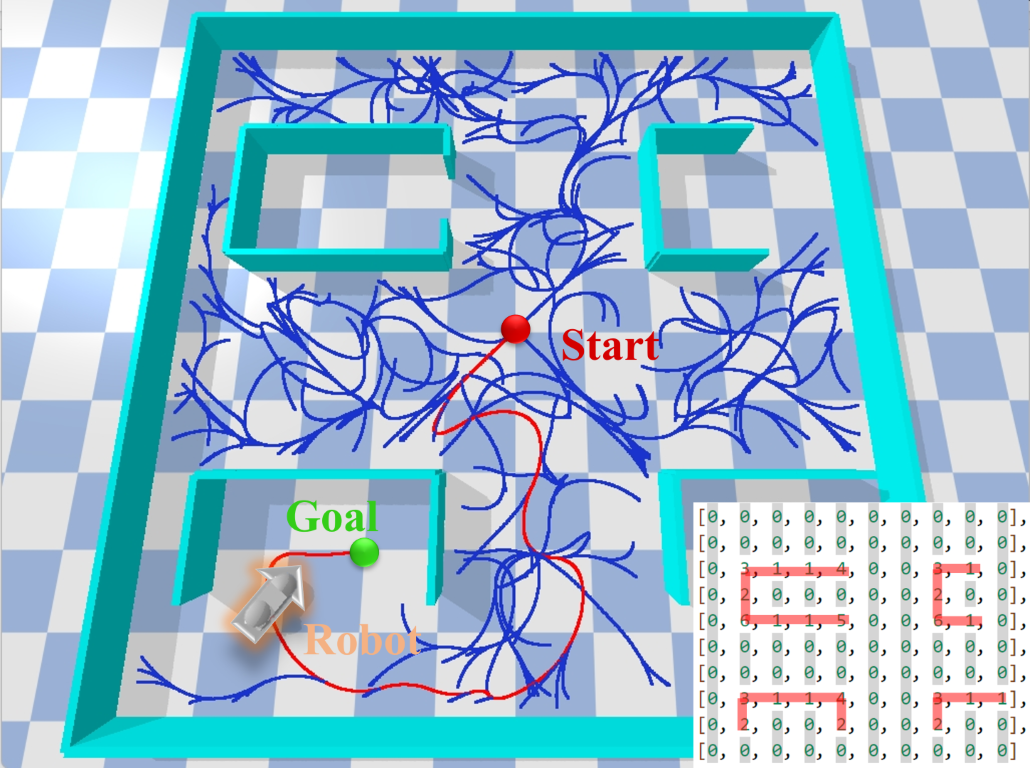
\includegraphics[width=0.9\columnwidth]{figures/env_setup.png}}
        \caption{The demonstration of the implemented kinodynamic RRT algorithm with a planar hovercraft robot model in PyBullet. The searched path is shown in red, the explored path is shown in blue and the configuration matrix of the maze is shown at the bottom right.}
        \label{fig:env}
\end{figure}


\section{Implementation}
% TODO Describe, in detail, using equations and illustrations where necessary, what you did to implement your project. 
% A block diagram showing the steps involved in the method is very helpful. 
% Make sure to discuss why you made the decisions you did.
In this section, the detailed implementation of the Kinodynamic RRT algorithm is discussed, outlining the specific steps and methodologies employed to address the complexities of kinodynamic planning.

\subsection{RRT Planner}

The RRT is an algorithm designed to efficiently search non-convex, high-dimensional spaces by randomly building a space-filling tree. The tree is constructed incrementally from samples drawn randomly from the search space and is inherently biased to grow towards large unsearched areas of the problem.

In order to build the tree and extract a path from goal to start once searched states are connected, a meta node is defined as a data class with two fields: state $\mathbf{x}$ and a pointer points to its parent node. The search tree $\mathcal{T}$ is a container build upon the meta nodes, with capabilities to query the nearest neighbor of a given node and add a given node as its vertex at the back end. Therefore, a general RRT path planning pseudo code is shown in Algorithm \ref{alg:rrt}.

\begin{algorithm}[htb]
    \caption{RRT Path Planning}
    \label{alg:rrt}
    \begin{algorithmic}
    \Require $x_{start}, x_{goal}$
    \Ensure PATH($\mathcal{T}.back()$)
    \State $\mathcal{T}.init(x_{start})$
    \For{$k=1 \textbf{ to } K$}
        \State $x_{rand} \gets $ RANDOM\_STATE()
        \State $x_{near} \gets \mathcal{T}.query(x_{rand})$ \Comment nearest neighbor
        \State $x_{prev} \gets x_{near}$
        \While{$True$}
            \State $x_{new} \gets $ EXTEND($\mathcal{T}, x_{prev}, x_{rand}$)
            \If {COLLISION($x_{new}$)}
                \State \textbf{break}
            \EndIf
            \State $\mathcal{T}.add\_vertex(x_{new})$
            \State $x_{prev} \gets x_{new}$
            \If {IS\_CONNECT($x_{new}, x_{rand}$)}
                \State \textbf{break}
            \EndIf
        \EndWhile
        \If {IS\_CONNECT($\mathcal{T}.back(), x_{goal}$)}
            \State \textbf{break}
        \EndIf
    \EndFor
    \end{algorithmic}
\end{algorithm}

\subsection{Dynamic Model}
To formulate the kinodynamic planning problem, a planar hovercraft robot model is used for demonstration. 

The dynamic model is defined as following.

\begin{itemize}
    \item Configuration space: $\mathbf q = [x, y, \theta]^T$
    \item State space (phase space): $\mathbf x = [\mathbf q, \dot{\mathbf{q}}]^T$
    \item Control input: $\mathbf u = [f_x, f_y, \tau_z]^T$
\end{itemize}

The continuous state space model
\begin{align*}
    \dot{\mathbf{x}}
    &= [\dot x, \dot y, \dot \theta, \ddot x, \ddot y, \ddot \theta]^T\\
    &= 
    \begin{bmatrix}
            \mathbf{0}_3 & \mathbf{I}_{3}\\
            \mathbf{0}_3 & \mathbf{0}_3
    \end{bmatrix}
    \mathbf{x} + 
    \begin{bmatrix}
        &\mathbf{0}_3& \\ 1/m&&\\ & 1/m&\\& & 1/I
    \end{bmatrix}
    \mathbf{u}\\
    &= \mathbf{A}\mathbf{x} + \mathbf{B}\mathbf{u}
\end{align*}
where $m$ is the mass of the robot and $I$ is moment of inertia.
The discretized state space model via forward Euler integration
\begin{align*}
    \mathbf{x}_{k+1} 
    &= \mathbf{x}_k + \dot{\mathbf{x}}_k dt\\
    &= (\mathbf{I} + \mathbf{A}dt)\mathbf{x}_k + \mathbf{B}dt\mathbf{u}_k\\
    &= \mathbf{A}_d \mathbf{x}_k + \mathbf{B}_d \mathbf{u}_k
\end{align*}
where $dt$ is the simulation time step.
However, a semi-implicit Euler method is used in the actual implementation, which can avoid the energy increment and leads to more accurate discretization, since it is the integration method used within PyBullet.
\begin{align*}
    \dot{\mathbf{q}}_{k+1} &= \dot{\mathbf{q}}_k + \ddot{\mathbf{q}}_kdt\\
    {\mathbf{q}}_{k+1} &= {\mathbf{q}}_k + \dot{\mathbf{q}}_kdt
\end{align*}

\subsection{Distance Metrics}

The choice of the metric for distance comparison between states has a strong effect on the likelihood of finding a solution. In kinodynamic planning, the standard Euclidean distances between two states often correspond poorly with the length of paths between two states. For example, moving sideways in a Dubins car requires performing "parallel parking" maneuvers that require moving a substantial distance forward and backward compared to the distance moved sideways\cite{hauser2020robotic}.

The ideal metric is the optimal cost to go from one state to another, but its computation is as difficult as the original planning problem.
Therefore, the weighted Euclidean distance is chosen to relieve this issue by manually tuning the weights of each individual state until a reasonable rate of convergence is observed.
\begin{align}
    dist(\mathbf{x}_1, \mathbf{x}_2) = \|\mathbf{W}(\mathbf{x}_1 - \mathbf{x}_2)\|_2
\end{align}
where $\mathbf{W}$ is a diagonal matrix with weights of state as its diagonal elements respectively.

\subsection{Applying Controls}

The EXTEND step in Algorithm\ref{alg:rrt} is formulated to find the optimal control input to minimize the distance between new states steered by motion primitives and the given target state $x_{rand}$, while observing the system dynamics $x_{new} = f(x_{near}, u_i)$.
\begin{align}
    &{u}^* = \min_{{u}_i} dist(f({x}, {u}_i), {x}_{rand})\\
    &{x}_{new} = f({x}, {u}^*) 
\end{align}
where $i=1, \dots, N$ and $N$ is the number of motion primitives. 

There are two ways to define a set of proper motion primitives.
One is, by heuristic, discretize the control space into grids and for each dimension, choose a unit control effort from $[-1, 0, 1]$ with a corresponding weight, then take a full combination of them. By adjusting the connectivity (e.g. 4-connect, 8-connect) of the discretized control space, we can have different number of primitives which represents different motion agility. Another way is to random sample $N$ primitives in range of the boundary of control inputs $\mathcal{U}$\cite{hauser2020robotic}. This method can save some parameter tuning effort since only $N$ is problem dependent, but the computation cost is also increased with the choice of $N$.

\subsection{Nearest Neighbor Search}

The nearest neighbor search is the most time expensive step in a RRT planner especially in high dimensional search problems. Since the convergence rate of RRT search is usually a bit random, use a search container with low time complexity of nearest neighbor query can greatly save the search time.

The most used data structure to find the nearest neighbor in high dimensions is the K-dimensional (KD) tree\cite{bentley1975multidimensional}.
The KD tree is a binary tree in which every node is a k-dimensional point. Every non-leaf node can be thought of as implicitly generating a splitting hyperplane that divides the space. The nearest neighbor of a query point can be determined with only $O(\log N)$ in time complexity, which is much faster than $O(DN^2)$ in brute force and independent with the state dimension $D$ (not computing the actual $D$ dimensional distance, but the parameters of separation hyperplanes).

However, building a static k-d tree from $N$ points takes $O(N \log N)$ complexity, and the number of data points is growing at every iteration. Note that most KD tree implementations do not provide the insertion or removing operations even through these operations take $O(\log N)$ time, but the re-balancing of the tree will harm the overall search performance. Therefore, the implemented RRT container utilize a lazy-rebuild strategy to further save the time costs of construction.

Instead of using only one KD tree and rebuild the tree in every iteration, a new vertex is inserted, an auxiliary $list$ is used to buffer new coming data points. The KD tree is rebuild in a lazy manner: only when the buffer list reaches the maximum buffer size. The nearest neighbor query is then divided into two steps, first query both the KD tree and the list (brute force), and then return the result with smaller distance.

\subsection{Steering between States}
In order to moving between two precise states, or "connect" between two tree nodes, a two-point boundary value problem (BVP) is formulated and solved locally as long as the distance between two states are smaller than a threshold\cite{lavalle2006planning}.
A 4th order collocation algorithm\cite{kierzenka2001bvp} is used to solve this BVP problem. The state and control input are concatenated as the extended state space $\mathbf{s} = [\mathbf{x}, \mathbf{u}]^T\in\mathbb{R}^9$ so that the dynamics $\dot{\mathbf{x}}=f(\mathbf{x}, \mathbf{u})$ can be viewed as a first order ODE system
\begin{align}
    \frac{d\mathbf{s}}{dt}
    & = f(t, \mathbf{s})
    = \begin{bmatrix}
        \mathbf{A}\mathbf{x} + \mathbf{B}\mathbf{u}\\
        \mathbf{0}_{3\times 1}
    \end{bmatrix}\\
    s.t.&\quad g(\mathbf{s}(a), \mathbf{s}(b))=\mathbf 0
\end{align}
where the boundary conditions $g(\cdot)$ drive the residuals between solution and boundary states to zero.

An important part of the process of solving the BVP is providing a guess for the required solution. The quality of this guess can be critical for the solver performance and even for a successful computation.
The initial guess of collocation states is the linear interpolation between the start and end states.

The steering between states via solving the BVP is used when the latest node of the search tree has already reached at a circle region in the task space (to simplify the problem, this region is assumed to have no obstacle) around the goal, so that it can provide a precise steered states to drive the robot to the goal.

\subsection{Bidirectional Planning}

The idea of bidirectional planning using RRT (Algorithm \ref{alg:bi-rrt}) is to grow two search trees with one rooted at the start and the other at the goal\cite{kuffner2000rrt}. At each iteration, both the start and the goal trees are extended toward a randomly sampled configuration. Then, if the trees are close enough, a connection will be attempted between them. If connected, the joined trees contain a unique path from the start to the goal.

However, in the kinodynamic planning problem, it is hard to "connect" arbitrary states even through both tree has overlapped edges. Thus, the BVP steering is used in a similar way as the single tree search but to connect nodes from both trees once the distance between them are smaller than a threshold\cite{lavalle2006planning}. Note that the $\mathbf{x}_{steer}$ is a list of steered states computed by the BVP solver.

\begin{algorithm}[htb]
    \caption{Bidirectional RRT Path Planning}
    \label{alg:bi-rrt}
    \begin{algorithmic}
    \Require $x_{start}, x_{goal}$
    \Ensure BI\_PATH($\mathcal{T}_a.back(), \mathcal{T}_b.back(), \mathbf{x}_{steer}$)
    \State $\mathcal{T}_a.init(x_{start})$
    \State $\mathcal{T}_b.init(x_{goal})$
    \For{$k=1 \textbf{ to } K$}
        \State $x_{rand} \gets $ RANDOM\_STATE($\mathcal{T}_a, \mathcal{T}_b$)
        \State $\mathcal{T}_a.connect(x_{rand})$
        \If {IS\_CONNECT($\mathcal{T}_a.back(), \mathcal{T}_b.back()$)}
            \State $\mathbf{x}_{steer} = BVP(\mathcal{T}_a.back(), \mathcal{T}_b.back())$
            \State \textbf{break}
        \EndIf
        \State SWAP($\mathcal{T}_a, \mathcal{T}_b$)
    \EndFor
    \end{algorithmic}
\end{algorithm}


\section{Results}

This section will demonstrate and analyze the performance of the kinodynamic RRT algorithm implemented in Python. The testing robot model is a planar hovercraft robot which has the ability to accelerate and decelerate in 2D positions and orientation (Figure \ref{fig:env}). The bidirectional variant of the kinodynamic RRT is also implemented and compared in terms of average path quality and computation time (Table \ref{tab:result}).

\begin{figure}[htb]
    \centering
        \textsf{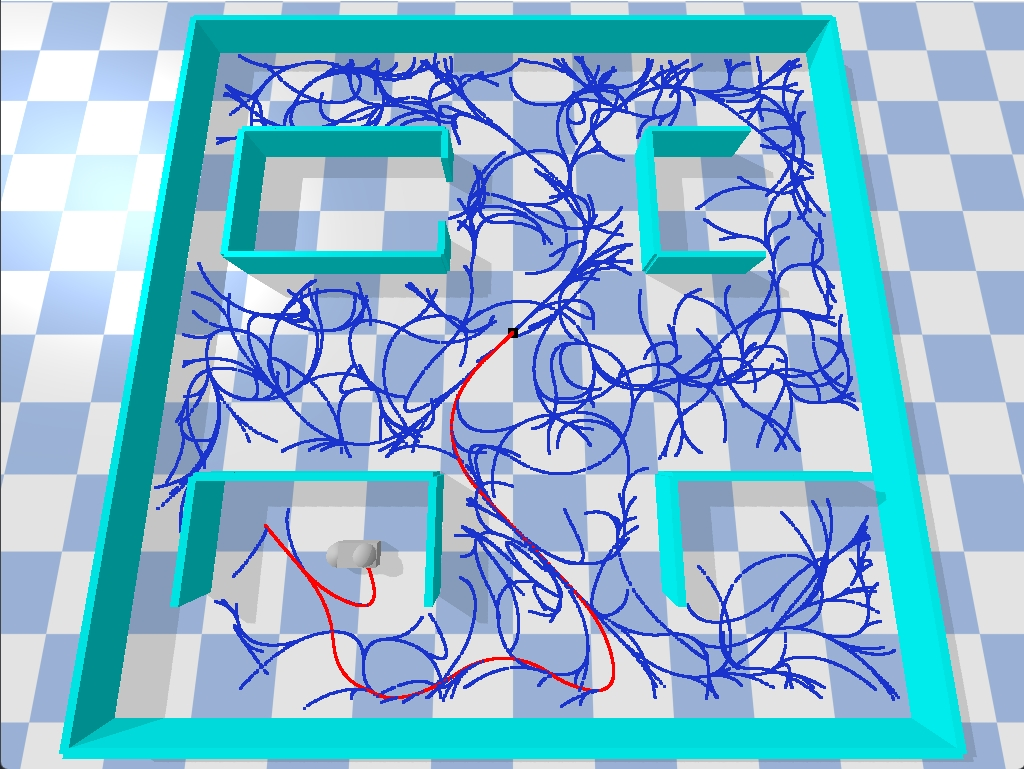
\includegraphics[width=0.9\columnwidth]{figures/KdRRT.png}}
        \caption{The visualization of the kinodynamic RRT. The searched path is shown in red, and the explored path is shown in blue.}
        \label{fig:kd-rrt}
\end{figure}

\subsection{Environment Setup}

The experiment environment is setup in the PyBullet\cite{coumans2016pybullet} a python module for robotics with real-time collision detection and multi-physics simulation\cite{coumans2015bullet}.

\subsubsection{Create the URDF of a hovercraft robot}
Omnidirectional movement control (i.e. planar joint) is not supported in PyBullet, and reset the base position and orientation of the robot is undesired and ill-posed when executing the planned trajectory.

The workaround is to created a fixed world link in the URDF, and connect three additional joints (two prismatic for positions and one continuous for orientation) to the robot body such that the 3 DOF of planar motion is retrieved.

\subsubsection{Track the planned trajectory via PD control}
Given the configuration of the robot is controllable through joint commands, the planned trajectory (treat as joint positions) can be executed via the build-in PD controller. In this way, the realistic physics execution of trajectory tracking can be observed.


\subsubsection{Build a custom 2D maze from json}
In order to build a generalized testing platform for the RRT based planning algorithms, a 2D maze builder from configuration file is implemented. A 10$\times$10 meter maze can be represented as a 2D matrix with numbers and edit through a simple $json$ file.

\subsection{Algorithm Evaluations}
% Try using different numbers of motion primitives and evaluate performance in terms of path quality and computation time for increasing numbers of primitives.

\begin{figure}[htb]
    \centering
        \textsf{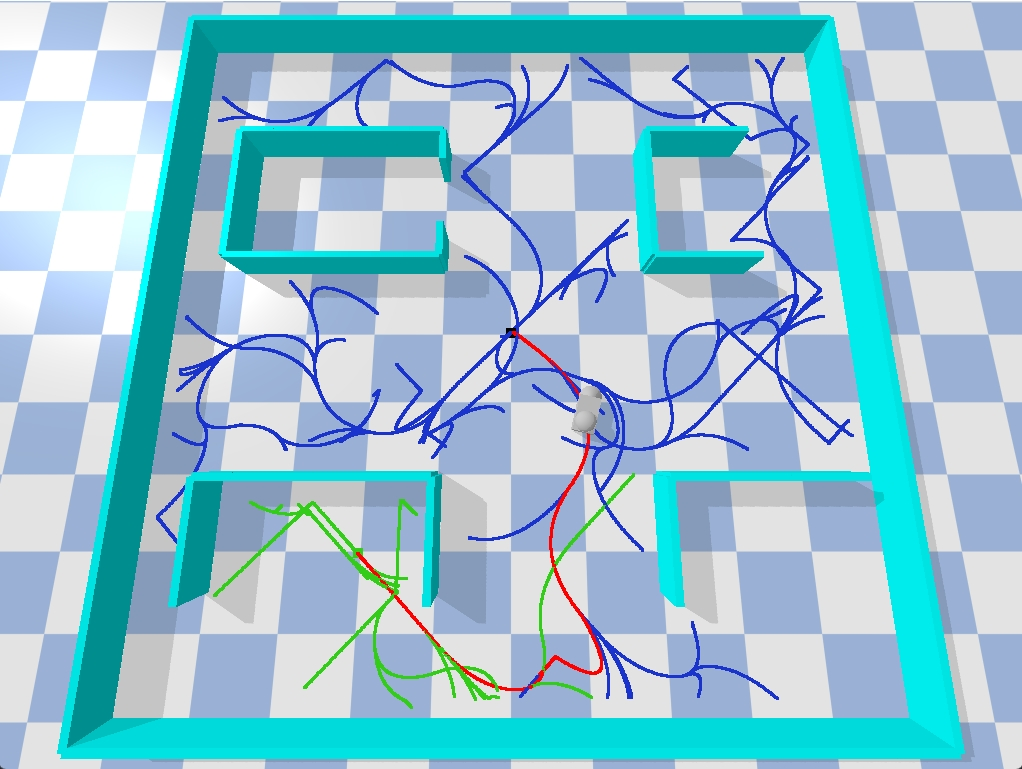
\includegraphics[width=0.9\columnwidth]{figures/BiKdRRT.png}}
        \caption{The visualization of the bidirectional kinodynamic RRT. The searched path is shown in red, the explored path of the start tree and the goal tree are shown in red and green respectively.}
        \label{fig:bi-kd-rrt}
\end{figure}

The mass $m$ of the robot is $1\ kg$, and its moment of initial $I$ is $1\ kg\cdot m^2$.
The state bounds $\mathcal{X}$ are in range of $[-10, 10]\ m$ for positions, $[-\pi, \pi]\ rad$ for orientation and $[-1, 1]\ m/s \text{ or } rad/s$ for linear and angular velocities.
The control bounds $\mathcal{U}$ are in range of $[-1, 1]\ N \text{ or } N\cdot m$ for force and torque.
The path quality is evaluated according the accumulated sum of the Euclidean distance between path waypoints $\sum \|\mathbf{q}_{i+1} - \mathbf{q}_i\|$.




\begin{table}[htb]
    \centering
    \caption{Performance Statistics for Various Examples}
    \label{tab:result}
    \begin{tabular}{@{}ccccccc@{}}
    \toprule
                             & No. of   & Random   & Path    & \multicolumn{3}{c}{Comput. Time (s)} \\ \cmidrule(l){5-7} 
    Algorithm                & Controls & Controls & Quality & Min        & Max        & Avg.       \\ \midrule
    \multirow{5}{*}{KdRRT}   & 6        & False    & 18.23    & 1.45        & 14.67        & 7.25        \\
                             & 26       & False    & \textbf{14.41}    & 3.24        & 22.55        & 8.99        \\
                             & 6        & True     & 29.46    & 2.41        & 21.49        & 10.78        \\
                             & 26       & True     & 20.71    & 0.75        & 36.25        & 7.54        \\
                             & 52       & True     & 18.73    & 2.28        & 11.42        & 5.93        \\\cmidrule(l){2-7} 
    \multirow{5}{*}{BiKdRRT} & 6        & False    & 19.10    & 0.21        & 3.05        & \textbf{1.71}        \\
                             & 26       & False    & 20.90    & 0.48        & 4.33        & 1.85        \\
                             & 6        & True     & 22.79    & 0.77        & 6.16        & 2.81        \\
                             & 26       & True     & 21.59    & 0.63        & 5.32        & 2.72        \\
                             & 52       & True     & 20.19    & 1.55        & 6.84        & 3.03        \\ \bottomrule
    \end{tabular}
\end{table}


Figure \ref{fig:kd-rrt} shows an example result of the searched path from the standard kinodynamic RRT, and Figure \ref{fig:bi-kd-rrt} shows another example result from the bidirectional variant of the kinodynamic RRT. The performance statistics of both algorithms are further studied and compared in Table \ref{tab:result}. All numbers, except the minimum and maximum, are calculated over the average of 10 times of execution. In terms of the number of motion primitives, 6 and 26 primitives stand for 4-connected and 8-connected discretization.


A few conclusions can be drawn  from Table \ref{tab:result}.
\begin{itemize}
    \item As the number of motion primitives increasing from 6 to 26, the path qualities of both algorithms are generally improved, but the average computation time become slower due to the increased amount of collision detections. 
    \item The bidirectional variant RRT can run about 3 times faster than the single tree version, but the quality of bidirectional searched path is usually worse than the path from standard search tree. The reason behind is that a bidirectional search will introduce more random states and both trees may connect at a point far from the optimal path from start to goal.
    \item The random uniform sampled motion primitives performs worse than the set of heuristic selected ones, also the convergence time is affected due to some portion of non-representative primitives.
\end{itemize}



\FloatBarrier
% \clearpage
% \nocite{*}
\bibliographystyle{IEEEtran}
\bibliography{ref.bib}

% \clearpage
\newpage
\appendix[Motion Planning Practice Software]

Taking the opportunity of this project, I extended the scope of my implementations to make it an starters friendly \href{https://github.com/silvery107/motion-planning-practice}{motion planning practice software}. Demonstration scripts are also extended to a KUKA iiaw robot arm with iterative inverse kinematics, and planned trajectory is tracked via the build-in PD controller.

Thanks to the ROB 422 course and Professor Dmitry Berenson, most implemented algorithms are taken from homeworks, but optimized for readability and efficiency.

\begin{figure}[htb]
    \centering
    \subfigure[RRT KUKA]{
        \textsf{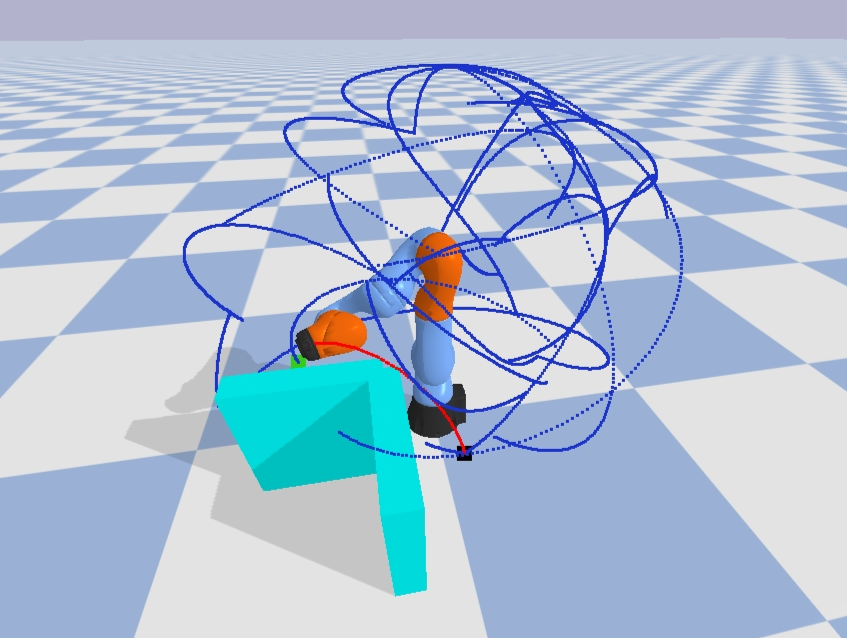
\includegraphics[width=0.44\columnwidth]{figures/kuka_rrt.png}}
    }
    \quad
    \subfigure[A*]{
        \textsf{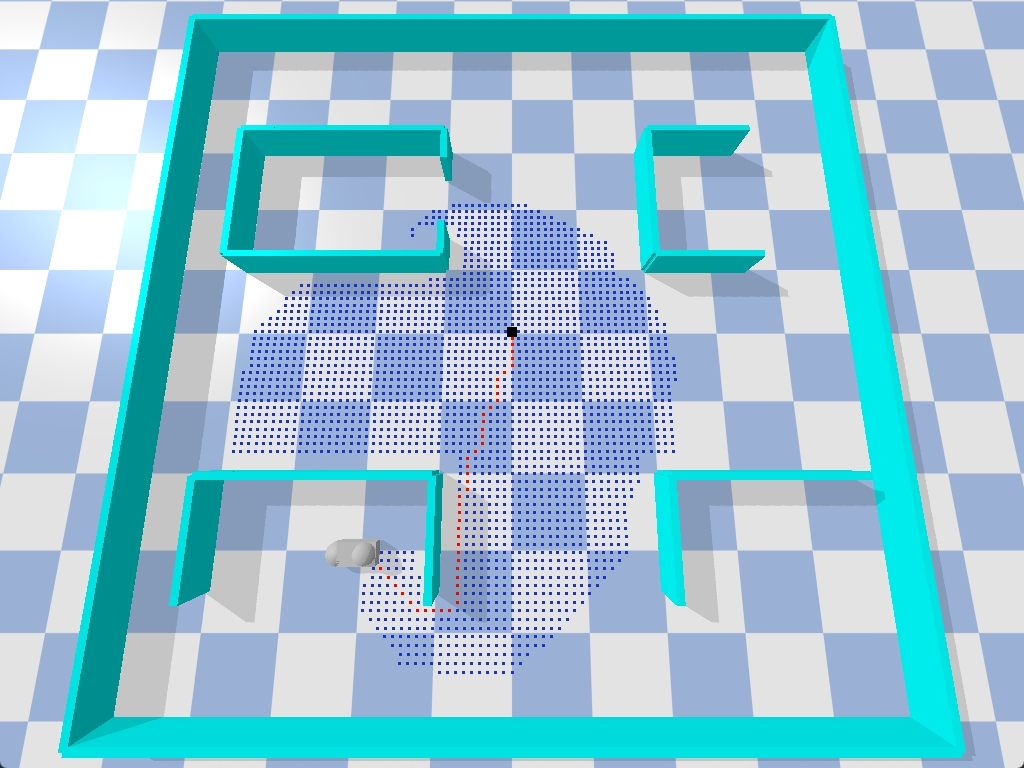
\includegraphics[width=0.44\columnwidth]{figures/Astar.png}}
    }
    % \caption{}
    % \label{fig:}
\end{figure}

\begin{figure}[htb]
    \centering
    \subfigure[RRT]{
        \textsf{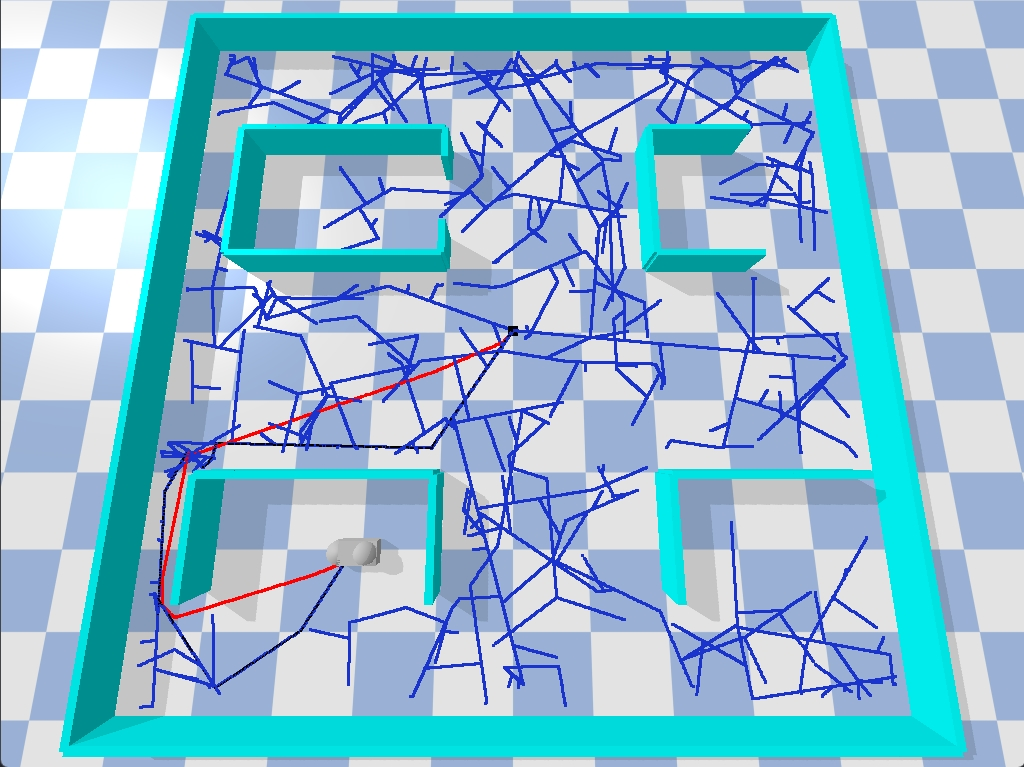
\includegraphics[width=0.44\columnwidth]{figures/RRT.png}}
    }
    \quad
    \subfigure[Bidirectional RRT]{
        \textsf{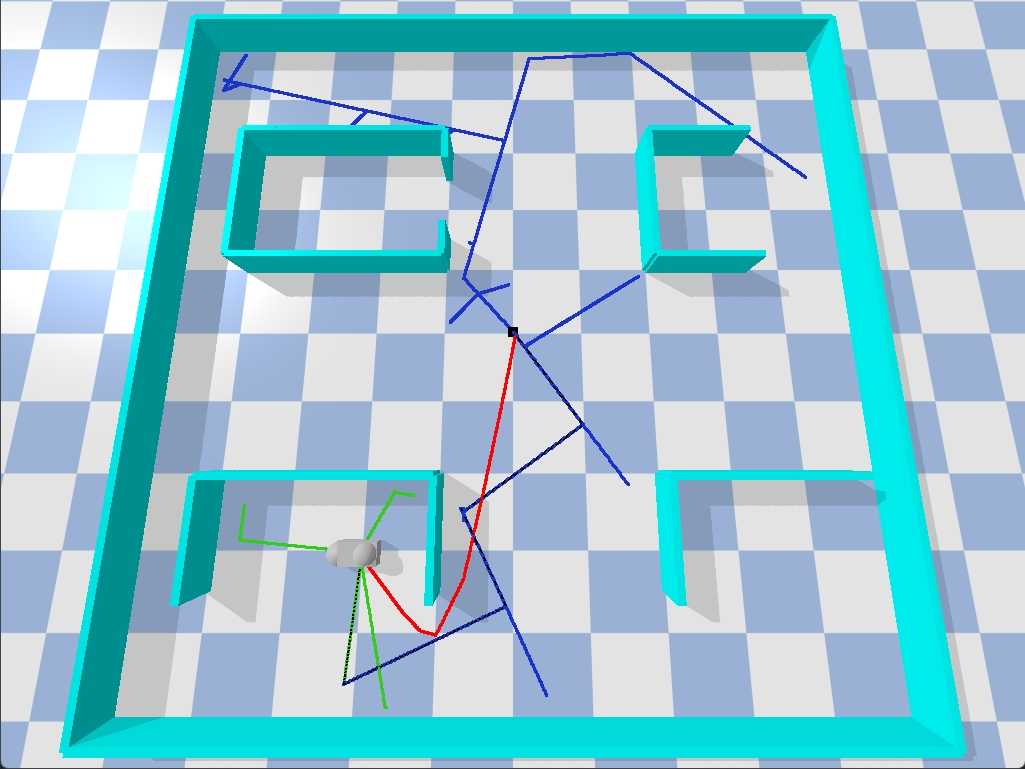
\includegraphics[width=0.44\columnwidth]{figures/BiRRT.png}}
    }
    % \caption{}
    % \label{fig:}
\end{figure}

\end{document}
